\documentclass[11pt]{scrartcl}
%%
%
% This is a poster template with latex macros and using
% the University of Florida Logo.  For further information
% on making postscript, resizeing, and printing the poster file
% please see web site 
% http://www.phys.ufl.edu/~pjh/posters/poster_howto.html
% 
% N.B. This format is cribbed from one obtained from the University
% of Karlsruhe, so some macro names and parameters are in German
% Here is a short glosary:
% Breite: width
% Hoehe: height
% sPALTE: column
% Kasten: box
%
% All style files necessary are part of standard TeTeX distribution
% On the UF unix cluster you should not need to import these files
% specially, as they will be automatically located.  If you
% run on a local PC however, you will need to locate these files.
% At UF try /usr/local/TeTeX...
% 
% P. Hirschfeld 2/11/00
%
% The recommended procedure is to first generate a ``Special Format" size poster
% file, which is relatively easy to manipulate and view.  It can be
% resized later to A0 (900 x 1100 mm) full poster size, or A4 or Letter size
% as desired (see web site).  Note the large format printers currently
% in use at UF's OIR have max width of about 90cm or 3 ft., but the paper
% comes in rolls so the length is variable.  See below the specifications
% for width and height of various formats.  Default in the template is
% ``Special Format",  with 4 columns.
%%
%% 
%% Choose your poster size:
%% For printing you will later RESIZE your poster by a factor
%%        2*sqrt(2) = 2.828    (for A0)
%%        2         = 2.00     (for A1) 
%%  
%% 
\def\breite{400mm}     % Special Format. 
\def\hoehe{400mm}      % Scaled by 2.82 this gives 110cm x 90cm 

%\def\breite{390mm}     % Special Format. 
%\def\hoehe{319.2mm}      % Scaled by 2.82 this gives 110cm x 90cm 
\def\anzspalten{2}
%%
%%\def\breite{420mm}     % A3 LANDSCAPE
%%\def\hoehe{297mm}
%%\def\anzspalten{4}
%%
%% \def\breite{297mm}     % A3 PORTRAIT
%% \def\hoehe{420mm}
%% \def\anzspalten{3}
%%
%% \def\breite{210mm}     % A4 PORTRAIT
%% \def\hoehe{297mm}
%% \def\anzspalten{2}
%%
%%
%% Procedure:
%%   Generate poster.dvi with latex
%%   Check with Ghostview
%%   Make a .ps-file with ``dvips -o poster.ps poster''
%%   Scale it with poster_resize poster.ps S
%%   where S is scale factor
%%     for Special Format->A0 S= 2.828 (= 2^(3/2)))
%%     for Special Format->A1 S= 2 (= 2^(2/2)))
%% 
%% Sizes (European:)
%%   A3: 29.73 X 42.04 cm
%%   A1: 59.5 X 84.1 cm
%%   A0: 84.1 X 118.9 cm
%%   N.B. The recommended procedure is ``Special Format x 2.82"
%%   which gives 90cm x 110cm (not quite A0 dimensions).
%%
%% --------------------------------------------------------------------------
%%
%% Load the necessary packages
%% 
\usepackage{palatino}
\usepackage[latin1]{inputenc}
\usepackage{epsf}
\usepackage{graphicx,psfrag,color,pstricks,pst-grad}
\usepackage{amsmath,amssymb}
\usepackage{latexsym}
\usepackage{calc}
\usepackage{multicol}
\usepackage{url}
%%
%% Define the required numbers, lengths and boxes 
%%
\newsavebox{\dummybox}
\newsavebox{\spalten}
%\input psfig.sty

%%
%%
\newlength{\bgwidth}\newlength{\bgheight}
\setlength\bgheight{\hoehe} \addtolength\bgheight{-1mm}
\setlength\bgwidth{\breite} \addtolength\bgwidth{-1mm}

\newlength{\kastenwidth}

%% Set paper format
\setlength\paperheight{\hoehe}                                             
\setlength\paperwidth{\breite}
\special{papersize=\breite,\hoehe}

\topmargin -1in
\marginparsep0mm
\marginparwidth0mm
\headheight0mm
\headsep0mm


%% Minimal Margins to Make Correct Bounding Box
%\setlength{\oddsidemargin}{-2.44cm}
%\addtolength{\topmargin}{-3mm}
\setlength{\oddsidemargin}{-2.44cm}
\addtolength{\topmargin}{-3mm}
\textwidth\paperwidth
\textheight\paperheight

%%
%%
\parindent0cm
\parskip1.5ex plus0.5ex minus 0.5ex
\pagestyle{empty}




\definecolor{recoilcolor}{rgb}{1,0,0}
\definecolor{occolor}{rgb}{0,1,0}
\definecolor{pink}{rgb}{0,1,1}





\def\UberStil{\normalfont\sffamily\bfseries\large}
\def\UnterStil{\normalfont\sffamily\small}
\def\LabelStil{\normalfont\sffamily\tiny}
\def\LegStil{\normalfont\sffamily\tiny}

%%
%% Define some commands
%%
\definecolor{JG}{rgb}{0.1,0.9,0.3}

\newenvironment{kasten}{
  \begin{lrbox}{\dummybox}
    \begin{minipage}{\linewidth}}
    {\end{minipage}
  \end{lrbox}
  \raisebox{-\depth}{\psshadowbox[cornersize=absolute,linearc=14pt,framesep=1em]{\usebox{\dummybox}}}\\[0.5em]}
\newenvironment{spalte}{
  \setlength\kastenwidth{1.2\textwidth}
  \divide\kastenwidth by \anzspalten
  \begin{minipage}[t]{\kastenwidth}}{\end{minipage}}

%\renewcommand{\emph}[1]{{\color{red}\textbf{#1}}}


%\def\op#1{\hat{#1}}
\begin{document}
%%%%%%%%%%%%%%%%%%%%%%%%%%%%%%%%%%%%%%%%%%%%%%%%%%%%
%%%               Background                     %%%
%%%%%%%%%%%%%%%%%%%%%%%%%%%%%%%%%%%%%%%%%%%%%%%%%%%%
{\newrgbcolor{gradbegin}{0.5 0.5 1}
  \newrgbcolor{gradend}{1 1 1}%{1 1 0.5}%
  %\rput[cm](15.23,-15){
  \rput[tl]{0}(0,0){
  \includegraphics[width=\paperwidth]{logos/antena1} %lower resolution
  %
\includegraphics[width=\paperwidth]{logos/alma_logo} %higher resolution
  }
\vfill}

%{\newrgbcolor{gradbegin}{0.5 0.5 1}%
%  \newrgbcolor{gradend}{1 1 1}%{1 1 0.5}%
%  \psframe[fillstyle=gradient,gradend=gradend,%
%  gradbegin=gradbegin,gradmidpoint=0.1](\bgwidth,-\bgheight)}
%\vfill
%%%%%%%%%%%%%%%%%%%%%%%%%%%%%%%%%%%%%%%%%%%%%%%%%%%%
%%%                     Header                   %%%
%%%%%%%%%%%%%%%%%%%%%%%%%%%%%%%%%%%%%%%%%%%%%%%%%%%%
\hfill
\psshadowbox{\makebox[0.95\textwidth]{%
    \hfill
	\parbox[c]{2cm}{
\includegraphics[width=2cm,height=!]{logos/alma_logo}}
    \hfill
    \parbox[c]{0.7\linewidth}{%
      \begin{center}
		\textbf{\Huge {Chilean Virtual Observatory services implementation for the ALMA public data}}\\[0.5em]
		\textsc{\large Jonathan Antognini$^{1}$, Mauricio Solar $^{1}$, Jorge Ibsen$^{2}$, Mauricio Araya$^{1}$,
				Lars Nyman$^{2}$, Diego Mardones $^{3}$, Camilo Valenzuela$^{1}$, Patricio Ramirez$^{1}$,
				Christopher Fernandez$^{1}$, Mario Garces$^{1}$
		\\[0.3em]
		{ $^1$Universidad T\'ecnicaFederico Santa Mar\'ia, Valpara\'iso, Chile}\\
		{ $^2$Atacama Large Milimeter/submilimeter Array, Santiago, Chile}\\
		{ $^3$}Universidad de Chile, Santiago, Chile}
      \end{center}}
	\hfill
    \parbox[c]{2cm}{
\includegraphics[width=3cm,height=!]{logos/usm_logo}}
	\hfill
\hfill}}\hfill\mbox{}\\

\hfill
\psshadowbox{\makebox[0.83\textwidth]{%
    \hfill
    \parbox[t]{0.8\linewidth}{%
\hfill{\large\bf{\color{red} Abstract}}\hfill\mbox{}\\
The success of an observatory is usually measured by its impact in the
scientific community, so a common objective is to provide transparent ways to
access the generated data. The Chilean Virtual Observatory (ChiVO), started
working in the implementation of a prototype, in collaboration with ALMA,
considering the current needs of the Chilean astronomical community, in
addition to the protocols and standards of IVOA, and the comparison of
different existing data access toolkit services. Based on this efforts, a VO
prototype was designed and implemented for the ALMA large scale of data. 
}
\hfill}}\hfill\mbox{}

\begin{lrbox}{\spalten}
  \parbox[t][0.61\textheight]{1.3\textwidth}{
   % \vspace*{0.2cm}
%%%%%%%%%%%%%%%%%%%%%%%%%%%%%%%%%%%%%%%%%%%%%%%%%%%%
%%%                 first column                 %%%             
%%%%%%%%%%%%%%%%%%%%%%%%%%%%%%%%%%%%%%%%%%%%%%%%%%%%
\begin{spalte}
     
	\begin{kasten}
        \section*{\hspace{0.2cm} {\color{red} Problem} }
		\begin{minipage}[t]{1.0\linewidth}
			Over time, observatories will start generating better quality data, in
			computational terms, with data sets in the order of the Tera- and Petabytes
			produced each year. This creates a series of problems, such as the
			distribution, access and processing of the data. This phenomena is known as
			"Astronomical Data Avalanche".
			
			In this context, the Chilean Virtual Observatory currently collaborates with
			ALMA observatory to promote compatible services with protocols and standards
			set by the International Virtual Observatory Alliance (IVOA). IVOA is an
			organization that discusses and sets the technical norms necessary to make a VO
			possible.
			
			Providing a web service under these conditions imposes a series of
			difficulties: capture and analyze the "use cases" and the requirements of an
			online data access platform; compare these needs to the IVOA protocols and
			standards; and finally implement a functional prototype that fulfills the
			previous requirements.
		\end{minipage} \hfill
\end{kasten}\hfill

	\begin{kasten}
        \section*{\hspace{0.2cm} {\color{red} ChiVO Architecture} }
			%\vspace{-0.1cm}
			\begin{minipage}{0.5\linewidth}
			ChiVO is a virtual observatory under construction
			that will host the data of the observatories located in Chile, adhered to the
			interoperability standards of the International Virtual Observatories Alliance
			(IVOA), and using last generation technologies.  
			Broadly, the architecture has three layers:
			\begin{itemize}
				\item \emph{Users}: \\astronomers and scientists in general, interested in the data published by the observatories
				\item \emph{Resources}: \\observatories and centres producing astronomical data (real or simulated)
				\item \emph{Intermediate layer}: \\defines what a virtual observatory is; that is, how users and resources communicate using protocols and standards to search and accees data.
			\end{itemize}
			%\emph{Users}:  astronomers and scientists in general, interested in the data
			%published by the observatories; \emph{Resources}: observatories and centres
			%producing astronomical data (real or simulated); \emph{Intermediate layer}:
			%defines what a virtual observatory is; that is, how users and resources
			%communicate using protocols and standards to search and accees data.
			\textbf{Requirements}\\\vspace{0.2cm}
			The creation of the ChiVO required the identification of the current needs of
			the national astronomy community, which can be summarized in:
			\end{minipage}
			\begin{minipage}{0.5\textwidth}
                        %\strut\vskip -\baselineskip
                        %\hfill
			\begin{center}
                        	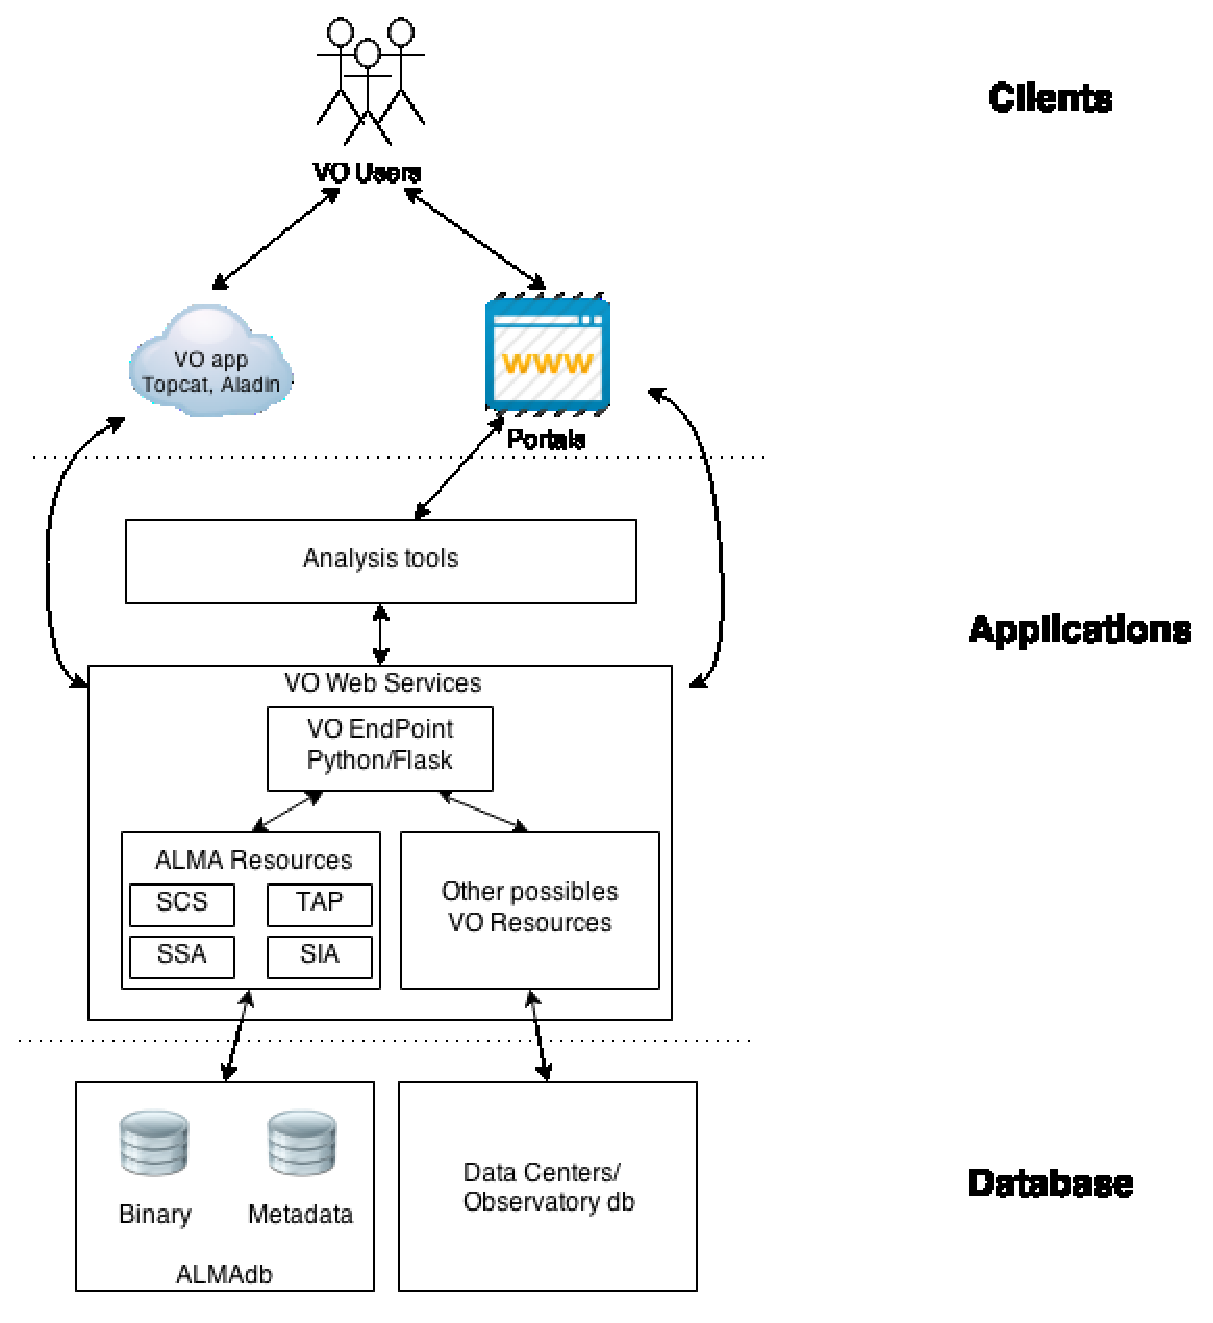
\includegraphics[width=0.8\textwidth]{img/chivo_capas}
			\end{center}
                        %\vspace{0.1cm}
                        \end{minipage}

\vspace{0.8cm}
                     \begin{minipage}[t]{0.3\linewidth}
                        \begin{itemize}
                            \item \emph{Discover:} Find astronomical data of an object or instrument on a high dimension
        specific region of the space, based on parameters of the spatial,
        temporary, spectral shafts, red shift, polarization, etc., either by
        search or exploration.
                        \end{itemize}
                        \end{minipage}
                        \begin{minipage}[t]{0.3\linewidth}
                        \begin{itemize}
                            \item \emph{Obtain:} A download link of the required data in different formats, either in
        		the VO or in an external service.
                        \end{itemize}
                        \end{minipage}
                        \begin{minipage}[t]{0.3\linewidth}
                        \begin{itemize}
                        \item \emph{Compare:} Information crossing of the data obtained between the different sources
        		of information.
                        \end{itemize}
                        \end{minipage}
			\\\vspace{0.3cm}
                     	\begin{minipage}[t]{1.0\linewidth}
			\vspace{0.3cm}
			A multidisciplinary team participated in this process (astronomers, engineers,
			scientists, experts in ALMA data, etc.); its duration was approximately 4
			months, while the astronomy community was defining its requirements, and the
			use cases, and IT team contrasted it with international standards.
			\end{minipage}
                        \\
	 \end{kasten}
    \end{spalte}
	 \hfill
%%%%%%%%%%%%%%%%%%%%%%%%%%%%%%%%%%%%%%%%%%%%%%%%%%%%
%%%               second column                  %%%             
%%%%%%%%%%%%%%%%%%%%%%%%%%%%%%%%%%%%%%%%%%%%%%%%%%%%
    \begin{spalte}
       
      \begin{kasten}
        \section*{\hspace{0.2cm} {\color{red} Progress Status} }
	\begin{minipage}[t]{1.0\linewidth}
		It was necessary to identify not only the requirements and use cases, but the
		interactions that users will have with the system, to begin the ChiVO
		development.  We can observe the interaction diagram sequence between the user
		and the ChiVO in figure.  According to this diagram, the
		requirements and technologies used will be specified in the progress status for
		each abstraction layer.

		The ChiVO software architecture is based on the use of the IVOA
		protocols and standards.  These protocols and standards are grouped in layers,
		with emphasis on the application and data layers; this, because their basic
		standards define the minimum operation that a VO should conduct.\vspace{0.3cm}
	\end{minipage}
	\begin{minipage}[t]{1.0\linewidth}
		\begin{center}
		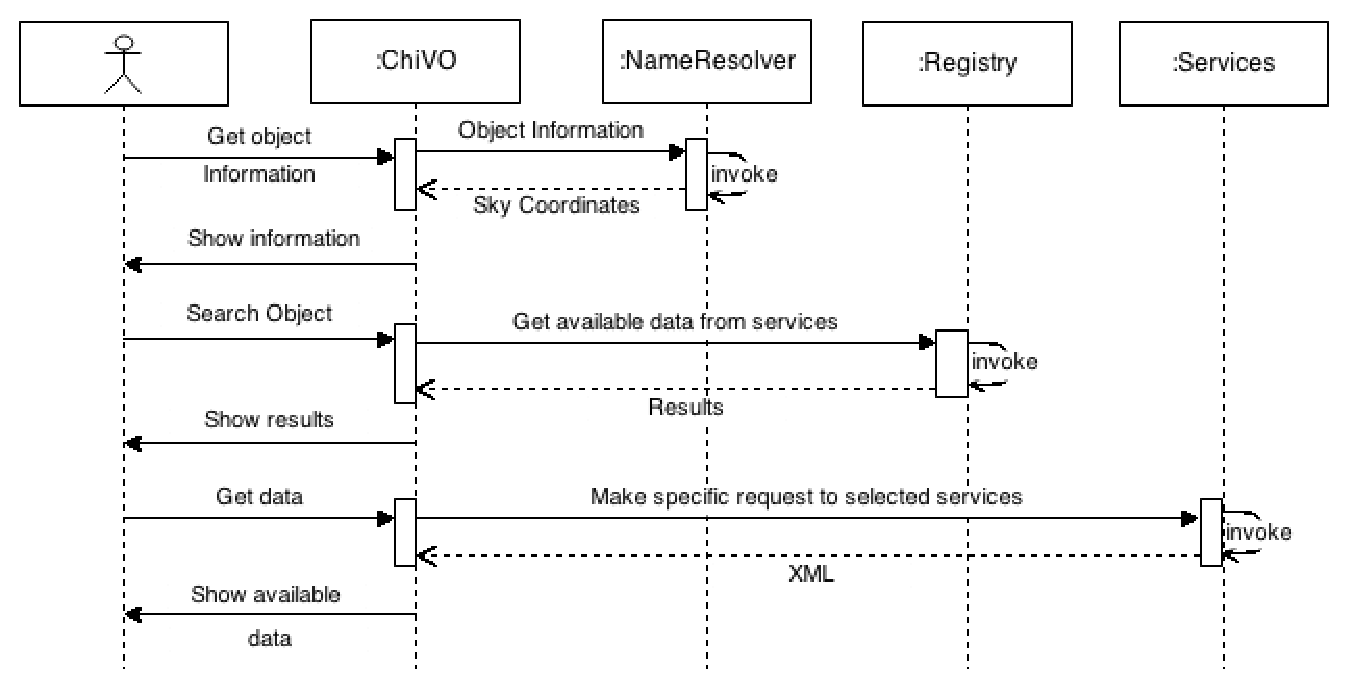
\includegraphics[width=0.9\textwidth]{img/secuencia}
		\end{center}
	\end{minipage}
	\begin{minipage}[t]{0.5\linewidth}
\textbf{Abstraction Layer:  Clients}\\\vspace{0.2cm}
Within the sequence diagram, the Frontend is the VO-Client; that is, it is in
charge of generating the interaction between users and other elements within
the system.
At the present, the frontend generated in RoR enables the interaction with:
\begin{description}
    \item Resolving names:\hfill \\
        from a name (String) returns the position of an object in celestial
        coordinates, using the SESAME service of Astrogrid.
    \item Registry: \hfill \\
        searches services within the endpoint, and then, according to the
        user's needs, it chooses on which to work for consultations.
    \item Services: \hfill \\
        consults with the different web services that provide data through a
        certain protocol, and standardizes the results in a XML VOTable for its
        organized deployment, using a VOView javascript library.
\end{description}
	\end{minipage}
	\begin{minipage}[t]{0.5\linewidth}
\begin{description}
\item \textbf{Abstraction Layer:  Applications} \hfill \\
The Endpoint is responsible for the generation of a transparent interaction
between the VO clients, and the possible resources that might be configured.
Here, the Endpoint generates an interface for services configured by the
Backend, and for those available, through the VO-Paris record.  VO-Paris has a
Web API in REST to consult for resources, returning a JSON file with outcomes.\\
\item \textbf{Abstraction Layer:  Data} \hfill \\
Currently, ALMA furnishes to the ChiVO public data, which include ASDM,
Measurement[2], FITS[3], however, it is necessary to draw out the ObsCoreDM metadata
to make possible their entry to the data base.
The procedure is carried out through a program, and using the DaCHS backend
framework, which enables the configuration of resources and services through
Resource Descriptor  configuration files.  Once created the entries in the data
base, and configured the SCS, SSAP, SIAP, TAP services, it can be accessed
through queries defined in each protocol.
\end{description}
	\end{minipage}
      \end{kasten}

    \end{spalte}
     \hfill\mbox{}
}

\end{lrbox}
\hfill
\resizebox*{0.95\textwidth}{!}{
  \usebox{\spalten}}\hfill\mbox{}

\vspace{1.0cm}
\hspace{1cm}
\psshadowbox[cornersize=absolute,linearc=14pt]{\makebox[0.923\textwidth]{%
 \hfill
 \parbox[t]{0.9\linewidth}{
\begin{minipage}[t]{0.95\linewidth}
\section*{ {\normalsize \color{red} Conclusions}}
{%\footnotesize
			\begin{minipage}[t]{0.50\linewidth}
Despite the amount of data generated by observatories in Chile, there was no VO
a year ago, and particularly, ALMA at the moment does not have services
compatible with VO. The implementation of the ChiVO caused a series of
complications that arise from the understanding of the needs of the
astronomers, and how these are translated to data systems and services, using
IVOA international regulations.

The approach of the current development is focused on incremental prototypes,
thus generating frequent deliverables to the system users (Astronomers) who are
pleased by the progress made. However, there are always things to implement, or
new ideas coming up. So far it has been possible to capture the astronomers
requirements, and to address the study of the protocols and standards, 
thus creating the data access services (SCS, SIA, SSA, TAP); 
			\end{minipage} \hspace{0.2cm}
			\begin{minipage}[t]{0.50\linewidth}
these have access to the data base that use a relational data model (ObsCore),
subjected to their own ChiVO architecture, which enables the interoperability
of the services.

Currently, the prototype is in its first delivery, and by mid-2014 it will be
launched its second iteration, which will include the public data of the cycle
0 of ALMA. Hence, more users will be familiarized with the system, having the
chance to test in situ the current functionalities and limitations of the
implementations. For the following versions it is considered the
implementation of other IVOA architecture protocols, as the section of Registry
and standards of access to resources, as VOSPace [1]. 
Regarding the models and multidimensional data, as the ALMA cubes, it will be
necessary to work in the creation or adaptation of the IVOA standards.
			\end{minipage}
}
\end{minipage}
}\hfill
}}\hfill\mbox{}\\
\vfill

\hfill
\psshadowbox{\makebox[0.95\linewidth]{
\hfill
\begin{minipage}[t]{0.30\linewidth}
	{\scriptsize
	{\small\bf Acknowledgements}
	
	\renewcommand{\baselinestretch}{0.4}
	This work is partially financed by the FONDEF D11I1060 project:
	``\emph{Development of an Astro-Informatic Platform for Management and Intelligent Analisys of Large-scale Data}''
	}
	
\end{minipage}\hfill

\begin{minipage}[t]{0.60\linewidth}
	{\scriptsize
	\renewcommand{\baselinestretch}{1.0}
	{\small\bf References}

        [1] Graham, Matthew and Harrison, Paul and Morris, Dave and Rixon, ``VOSpace service specification, Version 1.01'' (2007).
        \renewcommand{\baselinestretch}{0.5}

	[2] Petry, Dirk and others, ``Analysing ALMA data with CASA'' (2012).
	\renewcommand{\baselinestretch}{0.5}

	[3] Wells, DC and Greisen, EW and Harten, RH, ``FITS-a flexible image transport system'', Astronomy and Astrophysics Supplement Series (1981).
	\renewcommand{\baselinestretch}{0.5}
	}
\end{minipage}
}}\hfill\mbox{}

\hfill
\psshadowbox{\makebox[0.95\linewidth]{
\begin{minipage}[t]{0.15\linewidth}
	\begin{tabular}{cccc}
	
\includegraphics[width=!,height=1.5cm]{logos/alma} &
	
\includegraphics[width=!,height=1.5cm]{logos/fondef} &
	
\includegraphics[width=!,height=1.5cm]{logos/utfsm} &
	
\includegraphics[width=!,height=1.5cm]{logos/uchile} 
	\end{tabular}
\end{minipage} \hfill
\begin{minipage}[t]{0.50\linewidth}
	\begin{center}
	\Huge{Chilean Virtual Observatory}
	\end{center}
\end{minipage} \hfill
\begin{minipage}[t]{0.18\linewidth}
	\begin{tabular}{cccc}
	
\includegraphics[width=!,height=1.5cm]{logos/puc}
	
\includegraphics[width=!,height=1.5cm]{logos/reuna} &
	
\includegraphics[width=!,height=1.5cm]{logos/udec} &
	
\includegraphics[width=!,height=1.5cm]{logos/usach} &
	\end{tabular}
\end{minipage}
}}\hfill\mbox{}


\vfill
\hfill
{\scriptsize
Contact e-mail: {\color{blue}jantogni@csrg.cl} / For more information about
Chilean Virtual Observatory, please visit our web site
{\color{blue}http://www.chivo.cl}
}
\hfill
\

\end{document}
